% !TeX root = ../../tfg.tex
% !TeX encoding = utf8
%
%*******************************************************
% Construcción redes neuronales  
%*******************************************************
\section{Construcción \textit{Feedforward Network}}

TODO: Explicar nombre y que vamos a denotar a feedforward como redes neuronales de aquí en adelante. También comentar diferencia con perceptrón multicapa. 
% TODO añadir noción de que topológicamente son un grafo sin ciclos. 

Con el fin de facilitar la explicación partiremos de un ejemplo de un modelo básico en la sección \ref{rrnn:modelo_simple_rrnn}, para finalmente en la sección \ref{rrnn:construcción_generalizada} ofrecer una visión general. Además la evaluación de una red neuronal se realiza por un mecanismo conocido como \textit{forward propagation}, el cual 
describiremos en TODO :referencia y proceso de \textit{ aprendizaje} con una técnica conocida como \textit{back propagation} la cual se describe en TODO referencia. 

\subsection{Modelo básico de una red neuronal} \label{rrnn:modelo_simple_rrnn}
La información que se va a desarrollar a lo largo de esta 
sección proviene principalmente del capítulo cinco, páginas 227-256 del libro \cite{BishopPaterRecognition} y las notas online sobre redes neuronales de \cite{MostafaLearningFromData}.


\subsubsection*{Definición de la primera capa}
La primera capa está compuesta por $M$ combinaciones
lineales del vector de entrada $(x_1, \ldots, x_d)$
a las cuales denominaremos \textit{activaciones}

\begin{equation}
    a_j = \sum_{i=1}^D w_{ji}^{(1)} x_i + w_{j0}^{(1)}
    \text{ con } j \in \{1, \ldots, M \}.
\end{equation}
El superíndice (1) indica que los parámetro $w$ correspondientes pertenecen a la primera capa. 
Nos referiremos a los  parámetros $w_{ji}^{(1)}$ como 
\textit{pesos} y al parámetro $w_{j0}^{(1)}$ como 
\textit{sesgo}.  

\subsubsection*{Unidades ocultas}
Cada una de esas \textit{activaciones} será transformada
utilizando una \textit{función de activación} $h$ 
diferenciable y no linear

\begin{equation}
    z_j = h(a_j).
\end{equation}
En el contexto de las redes neuronales a $z_j$ se le conoce como \textit{unidad oculta} y que podrían ser de 
nuevo  transformados por una combinación lineal 
\begin{equation}
    a_k = \sum_{i=1}^M w_{ji}^{(2)} x_i + w_{k0}^{(2)}
    \text{ con } j \in \{1, \ldots, K \}.
\end{equation}
Nótese que ahora el tamaño de variables de entrada es $M$
y hay un total de $K$ unidades de activación, tanto $M$ como $K$ son
valores fijados por el diseñador de la red. 
Y combinando ambas capas resulta: 
\begin{equation}
    y_k(x,w) = \sigma 
    \biggl( 
        \sum^M_{j=1} w_{ji}^{(2)}
        h 
        \biggl(
            \sum_{i=1}^D w_{ji}^{(1)} x_i + w_{j0}^{(1)}
        \biggr)
        + w_{k0}^{(2)}
    \biggr) .
\end{equation}
Donde todos los pesos y sesgos han sido agrupados en el vector $w$. 

Si al vector de entrada se le añade una variable $x_0 = 1$, puede reescribirse cada expresión eliminando los sesgos y como producto vectorial

\begin{equation}
    y_k(x,w) = \sigma 
    \bigl(
         w^{(2)} \cdot
        h 
        \bigl(
             w^{(1)} \cdot x 
        \bigr)
    \bigr)
\end{equation}  

La función de activación $\sigma$ será escogida de acorde a la
naturaleza del problema, es decir \textit{cómo se desee codificar la salida}, por ejemplo si se trata de un problema de regresión, de clasificación, de probabilidad. 
 
De ahora en adelante trabajaremos con esta notación. 


En este ejemplo poseemos una capa oculta, 
puede definirse siguiendo esta misma idea
un red neuronal de múltiples capas ocultas. 

% Generalización de modelo 
\subsection{Construcción red neuronal de varias capas ocultas} \label{rrnn:construcción_generalizada}

Etiquetaremos a cada capa con $l \in \{0, \ldots, L \}$, donde $L+1$ es el número total de capas.  Donde 

\begin{itemize}
    \item La capa de entrada será la etiquetada con $l = 0$.
    \item La capa de salida que determina el valor de la red neuronal es la $l=L$.
    \item Las capas ocultas serán aquellas etiquetadas como $0 < l <L.$
\end{itemize}

Se usará un superíndice para hacer referencia a la capa. 
Cada capa posee un dimensión $d^{(l)}$, es decir que posee
$d^{(l)} + 1$ unidades o nodos. El nodo $d_0^{(l)}$ se trata del sesgo y siempre será uno. 

El modelo de red neuronal $\mathcal{H}_{n n}$ viene determinado una vez que se fija la arquitectura de la misma, es decir sus dimensiones $d$. 
\begin{equation}
    d = (d^{(0)}, d^{(1)}, \ldots, d^{(L)})
\end{equation}
y se tiene que cada red neuronal $h \in \mathcal{H}_{n n}$
viene determinada por sus pesos. 

\subsubsection*{Cálculo de una capa oculta}  
Cada nodo recibe una señal de entrada $s$ y determina una salida $x$. 
% Añadir gráfica   
La relación que existe entre dos nodos de capas contiguas es la siguiente: si $x_i^{(l-1)}$ es la salida de la unidad $i$ de la capa $l-1$, 
entonces se calcula la entrada de la unidad $j$ de la capa $l$ como 
\begin{align}\label{eq:construcción_red_neuronas:calculo_una_capa_oculta}
    s_j^{(l)} &= w_{i j}^{(l)} \cdot x_i^{(l-1)}  \\
    x_j^{(l)} &= \theta(s_j^{(l)})
\end{align}

Es decir, que en cada capa $l$ intervienen los siguientes elementos:  
\begin{table}[h]
    \begin{center}
    \begin{tabular}{| l | l | l |}
    \hline
    Elementos & Notación & Representación 
    \\ \hline
    Vector de entrada & $s^{(l)}$ &  Vector de dimensión $d^{(l)}$ \\
    Vector de salida & $x^{(l)}$ &  Vector de dimensión $d^{(l)}+ 1$ \\
    Pesos entrada & $W^{(l)}$ & Matriz de dimensiones $(d^{(l-1)}+1) \times d^{(l)}$ \\
    Pesos salida & $W^{(l+1)}$ 
    & Matriz de dimensiones $(d^{(l)}+1) \times d^{(l+1)}$ \\
    \hline
    \end{tabular}
    \caption{Elementos capa oculta $l$}
    \label{tab:rrnn_elementos_capa_oculta}
    \end{center}
\end{table}

\subsection{ \textit{Forward propagación}}
Sea $h \in \mathcal{H}_{n n}$ una red neuronal en esta sección explicaremos el algoritmo the \textit{forward propagation} para 
calcular el valor de $h(x).$

Gracias a la explicación anterior se puede apreciar que 
\begin{equation}
    x^{(l)} = 
    \left[ \begin{array}{c}
        1 \\
       \theta(s^{(l)})
        \end{array}
\right] .
\end{equation}
Donde $\theta(s^{(l)})$ es un vector de componentes $\theta(s^{(l)}_j)$. 
Para calcular el vector de entrada de la capa $l$, para cada nodo se hará
\begin{equation}
    s_j^{(l)} = \sum_{i=0}^{d^{(l-1)}} w_{i j}^{(l)}x_i^{(l-1)}.
\end{equation}
Que se formula para toda la capa como 
\begin{equation}
    s^{(l)} = W^{(l)} x^{(l-1)}.
\end{equation}
Y donde $x^{(0)} = x$ y por tanto $d^{(0)} = d.$
% Todo añadir ejemplo
Y por tanto la implementación del algoritmo sería

\begin{minted}{Julia}
#= Variables 
X_0 es el vector de entrada
W vector donde los elementos son los pesos de cada capa
=#
x = X_0  # Inicializamos 
for w in W   # Forward propagation
    x = [1; x] # Añadimos uno al principio
    s = w * s  
    x =  map(activation_function,x)
end
salida = x
\end{minted}
% Imagen red neuronal con pesos concretos
Veamos un ejemplo concreto para la siguiente red neuronal de la imagen \ref{img:construccion_rrnn:rrnn-2-3-2-1}
\begin{figure}[h!]
    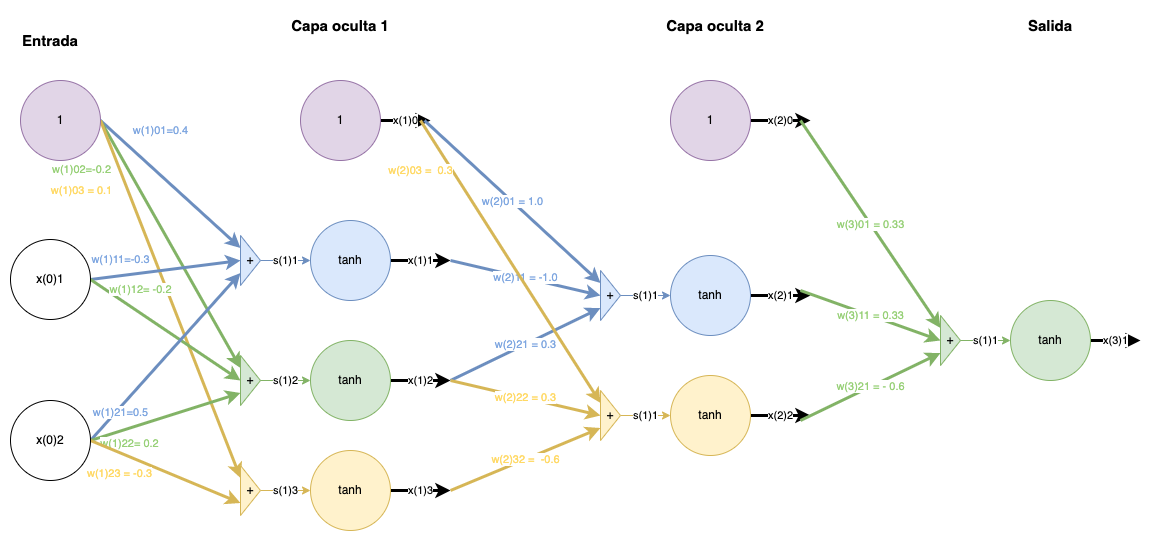
\includegraphics[width=\textwidth]{introduccion_redes_neuronales/construccion_redes_neuronales/rrnn-2-3-2-1-completa.png}
    \caption{Ejemplo de red neuronal con tres capas ocultas}
    \label{img:construccion_rrnn:rrnn-2-3-2-1}
\end{figure} 
Está compuesta por tres capas ocultas, el vector de entrada $x \in \R^2$, 
la primera capa oculta está compuesta por tres neuronas, la segunda por dos y la última, la salida por una. 
Las \textit{flechas} que conectan los nodos hacen referencia a los pesos de cada red neuronal. Por lo que para nosotros 
\begin{align}
    W^{(1)} = 
    \begin{bmatrix}
        0.4 & -0.3 & 0.5\\
        -0.2 & -0.2 & 0.2\\
        0.1 & 0 & -0.3
    \end{bmatrix} ,
    W^{(2)} = 
    \begin{bmatrix}
        1 & -1 & 0.3 & 0\\
        0.3& 0 & 0.3 & -0.6 
    \end{bmatrix} ,
    W^{(3)} = 
    \begin{bmatrix}
        0.33 & 0.33 & -0.6 \
    \end{bmatrix} 
\end{align}
Y si hacemos $x_0 = (1,0)$ y tomamos como función de activación
a la tangente hiperbólica, la ejecución del algoritmo queda reflejada en la tabla \ref{tab:construcción_rnnn:ejemplo_forward_propagation} resultando que 
$h((1,0)) = 0.439$.
\begin{table}[H]
    \begin{center}
\begin{tabular}{| c | c | c | c| }
    \hline
    Valor de $l$ &  $W^{(l)}$ & $\bigl(s^{(l)}\bigr)^T $ & $\bigl(x^{(l)}\bigr)^T$ \\ \hline
    0 & & & $(1,0)$ 
    \\ \hline
    1 & 
    $\begin{bmatrix}
        0.4 & -0.3 & 0.5\\
        -0.2 & -0.2 & 0.2\\
        0.1 & 0 & -0.3
    \end{bmatrix}$ 
    & $(0.1, -0.4, 0.1)$ & $(0.1, -0.38, 0.1)$
     \\ \hline
    2 & $\begin{bmatrix}
        1 & -1 & 0.3 & 0\\
        0.3& 0 & 0.3 & -0.6 
    \end{bmatrix}$
    & $(0.786, 0.126)$
    & $(0.656, 0.126)$
    \\ \hline
    3 & $\begin{bmatrix}
        0.33 & 0.33 & -0.6 
    \end{bmatrix}$ 
    & $(0.471)$ 
    & $(0.439)$
    \\ \hline
\end{tabular}
\caption{Ejemplo de ejecución del algoritmo de \textit{forward propagation}}
\label{tab:construcción_rnnn:ejemplo_forward_propagation}
\end{center}
\end{table}

\subsection{\textit{Backpropagation}}

Los parámetros que determinan una red neuronal son sus pesos, 
para actualizarlos utilizaremos la técnica de gradiente descendente. 
Que como ya explicamos consistía en \textit{avanzar} en dirección contraria a la del gradiente. 
\begin{equation}
    W(t+1) = w(t) - \eta \nabla E_{in}(w(t)). 
\end{equation}

Además, con el fin de reducir el coste del cálculo del gradiente, 
se utiliza el algoritmo conocido como \textit{backpropagation} que fue publicado en 
1989 en el artículo \cite{backpropagation-Hinton}. 

Sea $E_{in}(w)$ la función de error, la cual tomaremos como el error dentro de conjunto de entrenamiento, esto es,  si el conjunto 
de entrenamiento está constituido por $N$ datos de la forma $(x_n, y_n)$ con $x_n$ el vector de entrada y $y_n$ el estado o valor deseado para cualquier $n\in \{1, \ldots, N\}.$
\begin{equation}
    E_{in}(w) = \frac{1}{2} \sum^N_{n=1} e_n. 
\end{equation}
Para el cual 
\begin{equation}
    e_n = (h_w(x)- y_n)^2, 
\end{equation}
es una métrica para medir error entre, en nuestro caso  
la red neuronal $h_w$ y los valores deseados, con $w$ el vector que contiene las respectivas matrices de pesos de cada capa 
$W^{(l)} l \in \{1, \ldots, L\}.$  
%% Ejemplo 
Mostraremos un ejemplo primero antes de presentar el método general para facilitar la comprensión del algoritmo. 
% Imagen red neuronal simple
\begin{figure}[h!]
    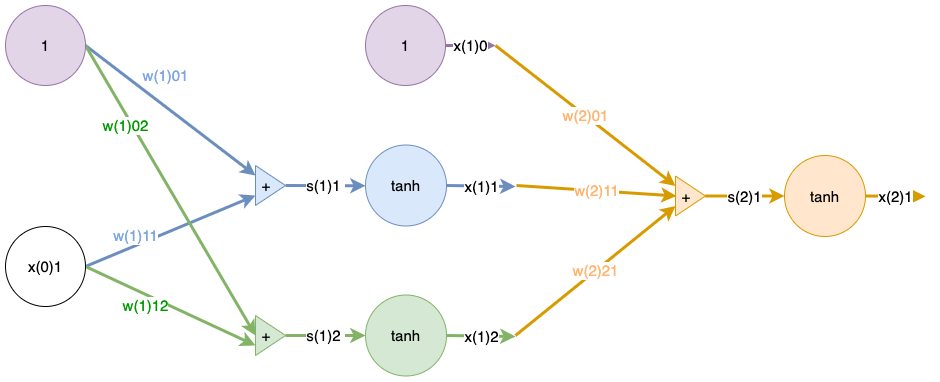
\includegraphics[width=\textwidth]{introduccion_redes_neuronales/construccion_redes_neuronales/rrnn-1-2-1.drawio.png}
    \caption{Ejemplo de red neuronal con tres capas ocultas}
    \label{img:construccion_rrnn:rrnn-1-2-1}
\end{figure} 
Queremos actualizar los pesos $w$ de la red neuronal 
$f_w : \R \longrightarrow \R$ presentada en \ref{img:construccion_rrnn:rrnn-1-2-1}.
$f_w$ está compuesta de dos capas ocultas. Supongamos que nos basaremos en un dato 
$(x, y)$ así pues podemos suponer que 
\begin{equation}
    E_{in}(w) = \frac{1}{2}e(f_w(x), y) = \frac{1}{2} (f_w(x)- y)^2.
\end{equation}
Como queremos actualizar los pesos utilizando el método de gradiente descendente necesitamos calcular el gradiente $\nabla E_{in}(w)$. 
En nuestro caso, $w=\{W^{(1)}, W^{(2)}\}$ con 
\begin{align}
    W^{(1)} = 
    \begin{bmatrix}
        w^{(1)}_{01} & w^{(1)}_{11} \\
        w^{(1)}_{02} & w^{(1)}_{12} \\
    \end{bmatrix} 
    \text{ y }
    W^{(2)} = 
    \begin{bmatrix}
        w^{(2)}_{01} & w^{(2)}_{11} & w^{(2)}_{21}\\
    \end{bmatrix}. 
\end{align}
Luego 
\begin{equation}
    \nabla E_{in}(w) = 
    \left(
        % primera capa 
        \frac{\partial e}{\partial w^{(1)}_{01}},
        \frac{\partial e}{\partial w^{(1)}_{11}},
        \frac{\partial e}{\partial w^{(1)}_{02}},
        \frac{\partial e}{\partial w^{(1)}_{12}},
        % segunda capa
        \frac{\partial e}{\partial w^{(2)}_{01}},
        \frac{\partial e}{\partial w^{(2)}_{11}},
        \frac{\partial e}{\partial w^{(2)}_{21}}
    \right).
\end{equation} 
Cada parcial se calcula, utilizando la regla de la cadena como
\begin{align}
    \frac{\partial e}{\partial w^{(1)}_{01}} 
    &=
    \frac{\partial e}{\partial s_1^{2}}
    \frac{\partial s_1^{2}}{\partial w^{(1)}_{01}} 
    \\
    &= 
    \frac{\partial }{\partial w^{(1)}_{01}}
         \tanh \left(s^{(2)}_{1}\right)
    \\
    &= 
    \left(1- \tanh^2 \left(s^{(2)}_{1}\right)\right) 
    \frac{\partial s^{(1)}_{1}}{\partial w^{(1)}_{01}}
    \\
    &= 
    \left(1- \tanh^2 \left(s^{(2)}_{1}\right)\right) 
    \frac{\partial }{\partial w^{(1)}_{01}}
    \left(w^{(2)}x^{(1)}\right)
    \\
    &= 
    \left(1- \tanh^2 \left(s^{(2)}_{1}\right)\right) 
    \frac{\partial }{\partial w^{(1)}_{01}}
    \left(
        \sum^2_{i=0}
        w^{(2)}_{i1}x^{(1)}_i
    \right)
    \\
    &= 
    \left(1- \tanh^2 \left(s^{(2)}_{1}\right)\right) 
    \left(
        \sum^2_{i=0}
        w^{(2)}_{i1}\frac{\partial x^{(1)}_i }{\partial w^{(1)}_{01}}
    \right)
    \\
    &= 
    \left(1- \tanh^2 \left(s^{(2)}_{1}\right)\right) 
    \left(
        \sum^2_{i=1}
        w^{(2)}_{i1}\frac{\partial }{\partial w^{(1)}_{01}}
        \left(
            \tanh \left(s^{(1)}_{i}\right)
        \right)
    \right)
    \\
    &= 
    \left(1- \tanh^2 \left(s^{(2)}_{1}\right)\right) 
    \left(
        \sum^2_{i=1}
        w^{(2)}_{i1}
        \left(
            \left(1- \tanh^2 \left(s^{(1)}_{i}\right)\right)
            \frac{\partial  }{\partial w^{(1)}_{01}}
            \left(
                \sum^1_{j=0}\sum^2_{k=1}
                w^{(1)}_{j k}x^{(0)}_j
            \right)
        \right)
    \right)
    \\
    &= 
    \left(1- \tanh^2 \left(s^{(2)}_{1}\right)\right) 
    \left(
        \sum^2_{i=1}
        w^{(2)}_{i1}
        \left(
            \left(1- \tanh^2 \left(s^{(1)}_{i}\right)\right)
            x^{(0)}_0
        \right)
    \right).
\end{align}
Notemos que no se han evaluado las apariciones de $s_i^{(j)}$.
Otro ejemplo sería
\begin{align}
    \frac{\partial e}{\partial w^{(2)}_{21}} 
    &=
    \frac{\partial }{\partial w^{(2)}_{21}}
         \tanh \left(s^{(2)}_{1}\right)
    \\
    &= 
    \frac{\partial }{\partial w^{(2)}_{21}}
         \tanh \left(w^{(2)}x^{(1)}\right)
    \\
    &= \left(
    1- \tanh^2 \left(s^{(2)}_{1}\right) \right)x^{(1)}_2.
\end{align}

Notemos que no se han desarrolla los términos de la forma $s^{(i)}_j$. Además si existen $Q$ pesos la complejidad del cálculo será $\mathcal{O}(Q^2)$, sin embargo, como hemos visto existen términos que se repiten en ambas ecuaciones, luego utilizando técnicas de 
programación dinámica y almacenando los valores que se repiten, 
reduciremos el coste a una complejidad de $\mathcal{O}(Q).$ Este 
algoritmo se le conoce como el de \textit{backpropagation}
basaremos su explicación en la publicada en
el artículo \cite{backpropagation-Hinton}.
%% Fin del ejemplo 
%% COMIENZA EL ARTÍCULO 

%Formalizaremos primero qué parámetros debemos estimar del gradiente.

Sea $\theta$ una función de activación derivable, 
 $L$ el número de capas ocultas, $N$ el tamaño del conjunto de entrenamiento $x^{(0)} = (1, x_1, \ldots, x_{d^{(0)}})^T$ 
siendo $x = (x_1, \ldots, x_{d^{(0)}})^T$ la entrada de la red neuronal, $x^{(L)}$ la salida de la red neuronal y 
$d^{(l)}$ la dimensión, número de nodos en la capa $l$-ésima. 
Recordemos que 
para cualquier $l \in \{1, \ldots, L\}$ con
\begin{equation}
    x^{(l)}
     = 
     \theta \left( s^{(l)}\right) 
     = 
     \theta \left( W^{(l)} x^{(l-1)}\right),
\end{equation}
y
\begin{equation}
    E(w) = \frac{1}{2} 
    \sum_{n = 1}^{N}
    \sum_{i = 1}^{d^{(L)}}
    \left({x_n}^{(L)}_i-y_{n_i} \right)^2
\end{equation}

%% Gradiente de la salida: 
Para simplificar la notación renombramos 
\begin{equation}
    E(w) = \sum^{N}_{n=1} e_n.
\end{equation}
y de ahora en adelante nos referiremos como $e$ a $e_n.$
Vamos a proceder a calcular primero los gradientes de la última capa, 
sea $w^{(L)}_{i j}$  con $j \in \{1, \ldots , d^{(L)}\}$, 
$i \in \{1, \ldots , d^{(L-1)}\}$  el peso que relaciona la salida 
$x_i ^{(L-1)}$ del  
nodo $i$ de la capa anterior con la entrada $s_j ^{(L)}$ del nodo $j$ de la última capa. 
Vamos a calcular $\frac{\partial e}{ w^{(L)}_{i j}}$ utilizando la regla de la cadena. 
\begin{equation}
    \frac{\partial{e}}{\partial w^{(L)}_{i j}}
     = 
     \frac{\partial{e}}{\partial x^{(L)}_j} 
     \frac{\partial x^{(L)}_j}{\partial s^{(L)}_j} 
     \frac{\partial s^{(L)}_j}{\partial w^{(L)}_{i j}}.
\end{equation}
Donde es fácil ver que para el tercer término
\begin{equation}\label{eq:backpropagation_s_última_capa_derivada}
    \frac{\partial s^{(L)}_{j}}{\partial w^{(L)}_{i j}}
    = 
    \frac{\partial }{\partial w^{(L)}_{i j}}
    \left(
        w^{(L)}_{\ast j } \cdot x^{(L-1)}
    \right)
    = 
    x^{(L-1)}_j
\end{equation}
Donde $w^{(L)}_{\ast j} = \left(w^{(L)}_{0 j}, w^{(L)}_{2 j}, \ldots, w^{(L)}_{d^{(L-1)} j}\right)$ representa los pesos correspondientes al nodo $j$,
 en forma de  vector fila y $x^{(L-1)} = \left(1, x ^{(L-1)}_1, \ldots, x ^{(L-1)}_{d^{(l-1)}}\right)^T$ el valor de la salida de la capa $L-1$
 en forma de vector columna.
 
 Por otro lado 
 \begin{equation}\label{eq:backpropagation_E_última_capa_derivada}
    \frac{\partial{e}}{\partial x^{(L)}_j} =
    x^{(L)}_j - y_j
 \end{equation}
 donde conocemos $x^{(L)}_j$ gracias al algoritmo de \textit{forward propagation}
 y $y_j$ la componente $j$-ésima del vector deseado en el entrenamiento.
y finalmente
\begin{equation}\label{eq:backpropagation_x_última_capa_derivada}
    \frac{\partial x^{(L)}_j}{\partial s^{(L)}_j} 
    = 
    \frac{d}{d s^{(L)}_j} 
        \theta \left( 
            s^{(L)}_j
        \right)
\end{equation}
que sabemos que se puede calcular por ser $\theta$ derivable y 
$s^{(L)}_j$ un valor conocido que ya ha sido calculado por el algoritmo de 
\textit{forward propagation.}

Por lo tanto, concluimos por 
(\refeq{eq:backpropagation_E_última_capa_derivada}),
(\refeq{eq:backpropagation_x_última_capa_derivada})
y  
(\refeq{eq:backpropagation_s_última_capa_derivada})
\begin{equation}
    \frac{\partial{e}}{\partial w^{(L)}_{i j}}
     = 
     \frac{\partial{e}}{\partial x^{(L)}_j} 
     \frac{\partial x^{(L)}_j}{\partial s^{(L)}_j} 
     \frac{\partial s^{(L)}_j}{\partial w^{(L)}_{i j}} 
    =
    \left( x^{(L)}_j - y_j \right) 
    \theta' \left( s^{(L)}_j\right)
    x^{(L)}_j.
\end{equation}
%%%% Gradiente interior 
Denotaremos por \textit{sensibilidad} a 
\begin{equation}
    \delta^{(l)} = \frac{\partial e}{ \partial s^{(l)}}.
\end{equation}

Para calcular la derivada de pesos de capas interiores $l \{1 \ldots L-1\}$
procederemos de la siguiente manera, para 
$j \in \{1, \ldots , d^{(l)}\}$ y 
$i \in \{1, \ldots , d^{(l-1)}\}$ 
\begin{equation}
    \frac{\partial{e}}{\partial w^{(l)}_{i j}}
     = 
     \frac{\partial e}{\partial s^{(l)}_j} 
     \frac{\partial s^{(l)}_j}{\partial w^{(l)}_{i j}}
    = 
    \delta^{(l)}
    \frac{\partial}{\partial w^{(l)}_{i j}}
    w^{(l) \cdot x^{(l-1)}}
    = 
    \delta^{(l)} x^{(l-1)}_i,
\end{equation}
donde  $x^{(l-1)}_i$ es conocida por el algoritmo de 
$\textit{forward propagation}$. por otra parte $\delta^{(l)}$ 
cumple que 
\begin{align}
    \delta^{(l)} 
    &= 
    \frac{\partial e}{\partial s^{(l)}}
    \\
    &= 
        \frac{\partial e}{\partial s^{(l+1)}}
        \frac{\partial s^{(l+1)}}{\partial s^{(l)}}
    \\
    &= 
    \delta^{(l+1)} 
    \otimes 
    \frac{\partial}{\partial s^{(l)}}
        \left( w^{(l)} \cdot \theta(s^{(l)})\right)
    \\
    &= 
    \delta^{(l+1)} 
    \otimes 
    w^{(l)} \cdot \theta'(s^{(l)}). 
\end{align}
\textcolor{red}{ Revisar penúltima operación.}
De esta manera a partir de las \textit{sensibilidades} de las 
capas posteriores es posible calcular las $l$-ésimas y puesto que 
la sensibilidad $\delta_{(L)}$ es conocida acabamos de determinar 
cómo calcular la derivada de todos los pesos  de manera constructiva. 
Procedemos a explicitar los cálculos. 




--------------------------------------------


%%  fin capa final
Comenzamos calculando $\frac{\partial E}{\partial \theta}$ para cada neurona de salida 
\begin{equation}
    \frac{\partial E}{\partial \theta} 
    = 
    \theta \left(s^{(L)}\right) - y.
\end{equation}
Aplicando la regla de la cadena podemos calcular $\frac{\partial E}{\partial s^{(L)}}$
para $j \in \{1,\ldots, d^{(L)}\}$
\begin{equation}
    \frac{\partial E}{\partial s^{(L)}_j} = 
    \frac{\partial E}{\partial \theta}
    \frac{d \theta}{d s^{(L)}_j}.
\end{equation}
Para un peso $w^{(l)}_j$
\begin{equation}
    \frac{\partial{E}}{\partial w^{(l)}_j}
     = 
     \frac{\partial{E}}{\partial s^{(l)}_j} 
     \frac{\partial s^{(l)}_j}{\partial w^{(l)}_j} 
    =
    \frac{\partial{E}}{\partial s^{(l)}_j} 
    \frac{\partial }{\partial w^{(l)}_j} 
        \left(W^{(l)} \cdot x^{(l-1)}\right)
    = 
    \frac{\partial{E}}{\partial s^{(l)}_j} x^{(l-1)}_j
\end{equation}
y finalmente para $l \in \{1, \ldots L-1\}$ 
\begin{equation}
    \frac{\partial E}{\partial \theta \left( s^{(l)}_i \right)}
    = 
    \frac{\partial E}{\partial \theta \left(x^{(l)}_i\right)}
    \frac{\partial x^{(l)}_i }{\partial \theta \left(s^{(l)}_i\right)}
    = 
\end{equation}

%% hasta aquí has llegado con el algoritmo
La entrada total de un nodo, $x_j$, es una función lineal de la salida anterior
\begin{equation}
    x_j = \sum_{i=1}^{d} \theta_i w_{i j}
\end{equation}

%%
Con el fin de abreviar notación llamamos \textit{sensibilidad} a
\begin{equation}
    \delta^{(l)}_i = \frac{\partial e}{\partial s^{(l)}_i}
\end{equation}
y puesto que $s^{(l)} = W^{(l)}x^{(l-1)}$
por la regla de la cadena resulta que 
\begin{equation}
    \frac{\partial e}{\partial W^{(l)}} 
    = % regla cadena
    \frac{\partial e}{\partial s^{(l)}}
    \frac{\partial s^{(l)}}{\partial W^{(l)}}
    = % s_s = w_s x_o
    \delta^{(l)}
    \frac{\partial }{\partial W^{(l)}}
    \left( W^{(l)} x^{(l-1)}\right)     
     = 
     \delta^{(l)}  x^{(l-1)}
\end{equation}
Por otro lado, teniendo en cuenta la topología de la red y que para 
el algoritmo de \textit{forward propagation} $x^{(l)}$ se calcula 
a partir de $x^{(l-1)}$, tendremos que $\delta^{(l)}$ se puede obtener gracias a $\delta^{(l+1)}$, siendo la relación: 
\begin{align}
    \theta(s^{(l)}
    = 
\end{align}
\begin{equation}
    \delta_j^{(l)}
    =
    \frac{\partial e}{\partial s^{(L)}_j}
    = % regla de la cadena
    \frac{\partial e}{\partial x^{(L)}_j}
    \frac{\partial x^{(K)}_j}{\partial s^{(L)}_j}
    = % sustituimos error
    \left( s^{(l)}_j \right)
    \frac{\partial e}{\partial x^{(L)}_j}
\end{equation}

\begin{equation}
    \nabla E_{in}(w) = 
    \left( 
        \frac{\partial E_{in}}{\partial W^{(1)}}, 
        \frac{\partial E_{in}}{\partial W^{(2)}},
        \ldots,
        \frac{\partial E_{in}}{\partial W^{(L)}}
    \right).
\end{equation}
Para cada entrada del vector
\begin{equation}
    \frac{\partial E_{in}}{\partial W^{(l)}}
    = \frac{1}{N} 
    \sum_{n=1}^N  \frac{\partial e_{n}}{\partial W^{(l)}}.
\end{equation}
Para calcular el valor de esta derivada usaremos la regla de la cadena, teniendo presente cómo se evalúa una capa a partir de la anterior,  $s^{(l)} = x^{(l-1)}W^{(l)}$ (\refeq{eq:construcción_red_neuronas:calculo_una_capa_oculta})

\begin{align}
    \frac{\partial e}{\partial W^{(L)}} 
    = 
    \frac{\partial e}{\partial s^{(L)}} 
    \frac{\partial s^{(L)}}{\partial W^{(L)}}
    = 
    \frac{\partial e}{\partial s^{(L)}} 
    x^{(L-1)}. 
\end{align}
Introduciremos esta notación 
\begin{equation}
    \delta^{(l)}
    =
    \frac{\partial e}{\partial s^{(l)}}.
\end{equation}

